%! TEX root = thesis.tex

\chapter{Research Study}%
\label{sec:researchstudy}


Through this chapter, we will set up our research study by identifying baselines for this problem, improve on the baselines by basing our study on related work discussed in the previous chapters, motivate the way forward towards our proposed architecture for the system. Through this process, we will build on existing research work, motivate our way forward and finally propose an architecture for us to compare results with existing systems.

Our research study will cover the following approaches and share results and discussions around the same. These results and literature reviews will motivate us towards our final architecture that we will discuss in the next chapter.

\begin{itemize}
    \item \textit{Zero Shot Prediction using State of the Art (SoTA) architectures.}
    \item  \textit{Singing Voice Separation Pre-processing for extracting vocal sections of the songs to boost the signal to the model}
    \item  \textit{Transfer Learning from current State of the Art (SoTA) architectures}
    \item  \textit{Domain Adaptation with Encoder - Decoder architectures}
\end{itemize}

Through the experiments, we will log the results and share the most promising approaches with relevant literature attached.


\section{Research and Experiments}%
\label{sec:experiments}

In order to build the research towards our end of objective of developing a strong songs to lyrics transcription algorithm, we will be starting with a baseline model that is based on the current state of the art techniques in this field. While there are no direct models that are defined for the field of Song Lyrics Transcription, the state of the art models will be inherited from the Speech domain (ASR), where OpenAI's Whisper and Wav2Vec2 architectures have been producing excellent results \cite{baevski2020wav2vec} \cite{radford2023robust}. Through the paper, when we refer to current state of the art models, we will be referring to Meta's Wav2Vec2.0 and OpenAI's Whisper models. We will be looking to model the problem we have defined in section \ref{sec:problemformulation}.The section will be structured in the form of questions and answers to help us answer the questions and motivate us towards a final architecture.

\subsection{How are Speech State of the Art Models (SoTA) performing for Song Lyrics Transcription in Zero Evaluation mode?}

    \begin{figure} [H]
    \centering
    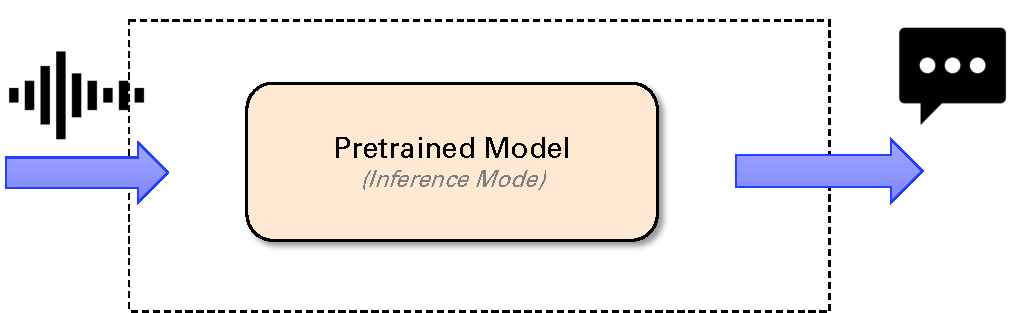
\includegraphics[width=0.9\textwidth]{05-research study/figures/zeroshot.pdf}
    \caption{Zero Shot Evaluation from Speech State of the Art Models  models}
    \label{fig:zeroshot}
\end{figure}

In this section, we will create the baseline for the Songs to Lyrics Transcription problem. Since there are is limited data available for songs to lyrics transcription and no direct Speech State of the Art Models  models that have been built for the songs to lyrics transcription problem, we will pick up the models from the speech domain and evaluate them in zero evaluation mode. This means that the model will be put in evaluation mode directly without any additional training as shown in Figure \ref{fig:zeroshot} and the data will be passed through them. In addition to that, there is a relatively less number of labeled data sources available for this domain. Therefore, our hypothesis is that the speech domain is a similar domain and there should be some capability to carry forward the learning without any additional training. For creating the baseline, we will send the test dataset to the models and calculate the word error rate (WER). To make the models in inference mode within PyTorch, the command \texttt{model.eval()} should be run prior to sending the data. By doing this, the layers are frozen and no back-propagation happens in the model. We leveraged the Huggingface implementation of the Wav2Vec2 model (with default weights) by using the following code block : \\
\begin{verbatim}
from transformers import AutoProcessor, AutoModelForCTC
model_backbone = "facebook/wav2vec2-large-960h-lv60-self"
processor = AutoProcessor.from_pretrained(model_backbone)
model = AutoModelForCTC.from_pretrained(model_backbone)
\end{verbatim}

The specific Wav2Vec2 that was pulled for our baseline model was the Large model that was pre-trained on 960 hours of Librispeech and Libri-Light datasets at 16KHz audio. Once trained, the model was finetuned on the same 960 hours of audio dataset in a labelled fashion with the pre-trained component in evaluation model . This particular model was trained using the Self-Training Objective. Self-training objective represents the fact that an initial acoustic model is trained on available labeled data and then the unlabelled data is inferenced to produce pseudo labels. This is typically done multiple times in Self-training till the entire network converges. In Wav2Vec2, self-training objective is implemented by pre-training the Wav2vec2 model on unlabeled data, use the model to label the unlabelled data and finally use the pseudo labeled data to train the final model \cite{xu2021self}. This model has 315 Million parameters and is the largest Wav2vec2 model. Since, this model is well suited for the Speech domain and produces Speech State of the Art Models  results of 1.8/3.3 Word Error Rate for the Librispeech benchmark, this was selected. On the Whisper model front, the model selected was \texttt{openai/whisper-large-v2}. This is the largest whisper model with the best performance in the speech domain. The Whisper Large V2 model has 1550 Million parameters in the model. This is imported with default weights into our process through the HuggingFace implementation as follows:

\begin{verbatim}
from transformers import AutoProcessor, AutoModelForSpeechSeq2Seq
model_backbone = "openai/whisper-large-v2"
processor = AutoProcessor.from_pretrained(model_backbone)
model = AutoModelForSpeechSeq2Seq.from_pretrained(model_backbone)
\end{verbatim}

We calculate the Word Error Rates by utilizing the \texttt{jiwer} \cite{morris2004and} python library.  The below table gives a summary of the performance of the Speech Models.


\renewcommand{\arraystretch}{2}
\setlength{\arrayrulewidth}{0.3mm}
\begin{table}[H]
\small
\begin{center}
\begin{tabular}{ |p{7cm}| p{3cm}| p{4cm} | }
\multicolumn{3}{c}{Inference done on \texttt{DALI-validation}} \\
\cline{1-3}
 Models     & WER  & Experiment-1 WER \\
\hline  \hline
 \textit{Wav2Vec2 Large Self}               &                 0.956  &   \\
 \textit{Whisper Large}                     &         \textbf{0.854} & \\
\hline  \hline
\end{tabular}
\caption{\label{zeroshot} Zero Shot Performance of Speech State of the Art  models}
\end{center}
\end{table}


From the above table, we can see that Whisper outperforms the Wav2Vec2 model considerably. This could be attributed to two reasons -  (1) The Whisper model has been trained on significantly larger amount of labeled data. There is a good chance that the data that was considered for this problem is part of the training set and hence, the domain is represented better in this model. (2) The Whisper model is a encoder-decoder architecture and there is a rigorous decoding procedure that is taken into account by Whisper to make the right decision on how to decode. Consequently, the decoding procedure is more robust than that of the generic CTC decoding that Wav2Vec2 employs.


The  Word Error Rate (WER) metric for songs to lyrics transcription as seen above in table \ref{zeroshot} show that the metric is significantly higher than their counterparts in the speech domain, where the best WER reported in the papers are \textit{0.033}. Hence, the songs do not directly transfer very well and cannot be reliably used as a direct solution to the problem. In the next section, we outline the hypothesis of understanding the key difference between speech and songs and finding a way to bridge the gap through pre-processing.

\subsection{Does Singing Voice Separation improve the State of the Art?}

Songs contain both the vocal and music components within them. However, for lyrics generation, the music components (such as Piano, Guitar etc.) can be considered as noise as they do not contain the information required for transcribing into lyrics. Hence, in this particular section, our hypothesis is to test whether we can look at techniques outlined in section \ref{sec:demucs} to separate the vocals from the rest of the music. To do this, we take the current State of the Art model in singing voice separation called the Hybrid DEMUCS algorithm to extract only the vocal component from the song. To separate the vocals, we leveraged the \texttt{--two-stems=vocals} option within the DEMUCS framework, allowing us to extract the vocals from other music.

\begin{figure}
    \centering
    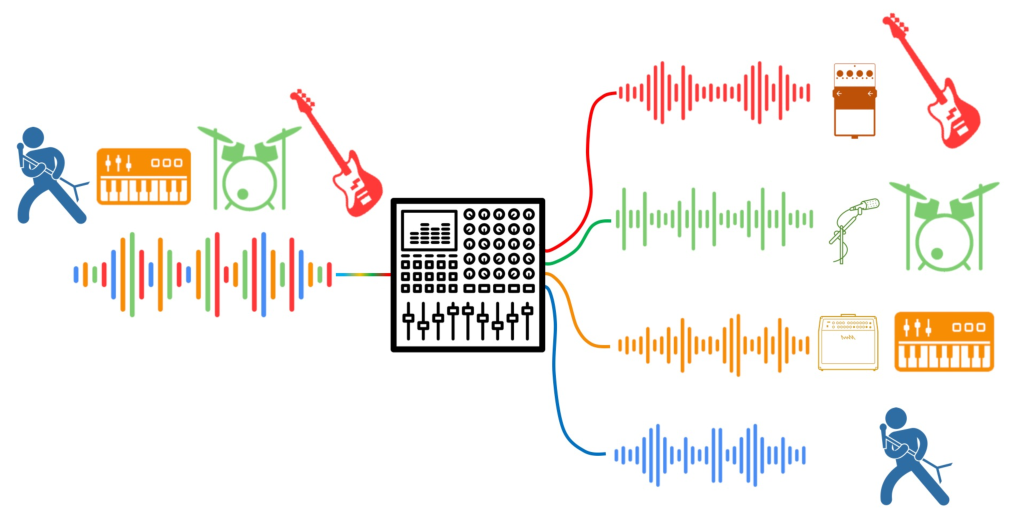
\includegraphics[width=0.8\textwidth]{05-research study/figures/sourceseparation.pdf}
    \caption{Music Source Separation (Vocal Separation) \cite{opensourceseparation:book}}
    \label{fig:musicsourceseparation}
\end{figure}

The table \ref{demucsperformance}  shows that there is a significant improvement from the non-DEMUCS version shown in table \ref{zeroshot} (\textit{0.851 vs 0.956 for Wav2vec2 and 0.677 vs 0.854 for Whisper}). This performance boost can be seen in both of the architectures, allowing us to confirm our hypothesis that the instruments were indeed adding unwanted noise to the vocals and it resulted in lyrics extraction to become a much more difficult problem. The performance improvement from Whisper model is impressive as it improves by more than 0.177  Word Error Rate on the validation dataset. \\


\renewcommand{\arraystretch}{2}
\setlength{\arrayrulewidth}{0.3mm}
\begin{table}[H]
\small
\begin{center}
\begin{tabular}{ |p{7cm}| p{3cm}| }
\multicolumn{2}{c}{Inference done on \texttt{DALI-validation}} \\
\cline{1-2}
 Models     & WER  \\
\hline  \hline
 \textit{Wav2Vec2 Large Self + SVS}    & 0.851 \\
 \textit{Whisper Large + SVS}   & \textbf{0.677} \\
\hline  \hline
\end{tabular}
\caption{\label{demucsperformance} Performance of Vocal Separation with baseline models}
\end{center}
\end{table}


Evaluating the performance of DEMUCS, we can see through auditory inspection a clean vocal separation for majority of the songs. However, there are also cases where the entire vocal component has been misclassified as music instrument and removed from the vocal separated audio, and also cases where there is leakage from the instruments to the vocal component. Since we use the algorithm merely to separate the audio and not delve into the robustness of the approach, we are not evaluating the performance of DEMUCs on our dataset. A future improvement that can be done for this, that could further improve the results at the risk of increasing model complexity is to perform source separation only when it is useful. This could be achieved by training a classifier to predict whether source separation would be successful or not by looking at the spectrogram.


\subsection{Does Transfer Learning further improve the solution?}

    \begin{figure} [H]
    \centering
    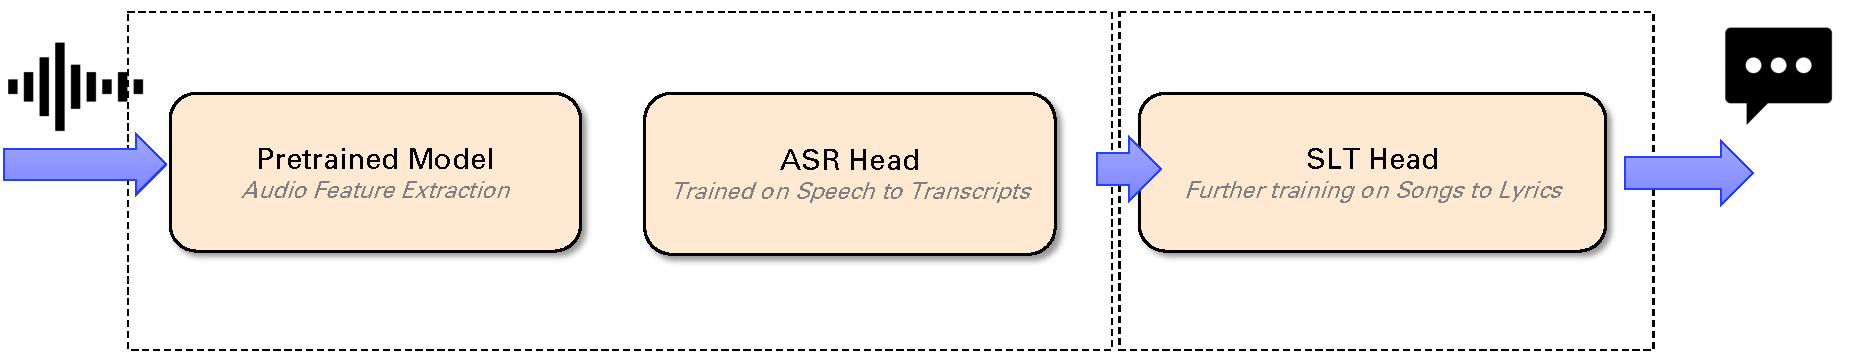
\includegraphics[width=1.0\textwidth]{05-research study/figures/transferlearning.pdf}
    \caption{Transfer Learning}
    \label{fig:transferlearning}
\end{figure}

In this section, we will pick up from the conclusions of the previous research question. In a zero shot setting with source separation, we are already seeing improvements in both the architectures from the baseline. One of the challenges with songs data is that, the lyrics are not always fully formed sentences such as speech or are spoken with contractions and expansions to make musical effect. Hence, there is a discernible shift in the domain between the speech domain and songs domain. In order to improve the domain knowledge of the model into the songs domain, we will look into transfer learning approaches that can leverage the information learnt in the existing speech domain and learn more about translating the features into the song domain.
Transfer learning is the approach where features generated from one problem are applied to a different problem statement. This initial problem could be similar or be in a completely different setting dependent on the approach in which transfer learning is applied. In our case, we are still interested in the audio inputs to text transcription output, which is similar to the speech domain. Hence, we will leverage the fine-tuning approach of transfer learning. This is a well documented approach for learning on tasks where there is less data as seen here \cite{buragohain2022deep} \cite{hosna2022transfer}


In our transfer learning studies, we will apply transfer learning through the following approach :
\begin{itemize}
    \item We will take the pre-trained or trained model and freeze the parameters to not allow further learning/training.
    \item We will unfreeze the Language Modeling head (LM), which is a series of layers that are on top of the models that allow for translation into the problem statement.
    \item We will fine-tune the model with new data. The learning will affect the language model or top layers only, while keeping the base model intact. This ensures that the feature generation part is not affected but the translation into lyrics from the audio songs is better represented in our songs to lyrics transcription (SLT) model.
\end{itemize}

In our particular method, we will fine-tune the models using PyTorch Lightning and Huggingface. The Wav2vec2 finetuning was done using Microsoft's DeepSpeed's implementation of \texttt{freeze-unfreeze-10} , where the first 10 epochs had the model and backbone frozen with no learning happening. The next 5 epochs were unfrozen, allowing for the features to be learnt well. The optimizer used was the AdamW optimizer and this provided the best results for the fine-tuning procedure. The Whisper model was fine-tuned using the HuggingFace Seq2SeqTrainer implementation. Both were trained with EarlyStopping for 15 Epochs. While the Wav2Vec2 ran for the entire 15 Epochs, Whisper quickly converged to the optimum results shown above in 2 epochs. The learning rates were \texttt{1e-05} and \texttt{batchsize = 4} for both the models. The results obtained from the study are shown in table \ref{transferlearning-performance-table}

\renewcommand{\arraystretch}{2}
\setlength{\arrayrulewidth}{0.3mm}
\begin{table}[H]
\small
\begin{center}
\begin{tabular}{ |p{7cm}| p{3cm}| }
\multicolumn{2}{c}{Inference done on \texttt{DALI-validation}} \\
\cline{1-2}
 Models     & WER  \\
\hline  \hline
 \textit{Wav2Vec2 Large Self + SVS + TL}    & 0.7416  \\
 \textit{Whisper Large Self + SVS + TL}   & \textbf{0.607}  \\
\hline  \hline
\end{tabular}
\caption{\label{transferlearning-performance-table} Summary of Transfer Learning (Fine-tuning)}
\end{center}
\end{table}


The results clearly show the improvement due to Transfer Learning on the two architectures. Both of them are significantly able to better understand the songs domain than the initial zero shot model that was created. By fine-tuning, we are able to see models show significant improvement than the successful experiment shown with SVS included \ref{demucsperformance} (\textit{0.7416 vs 0.851 for Wav2vec2 and 0.607 vs 0.677 for Whisper}). Therefore, Transfer learning can be successfully seen as an improvement to the existing methodology for learning features that are significant to the songs domain.


\begin{figure} [H]
     \centering
     \begin{subfigure}[b]{0.49\textwidth}
         \centering
         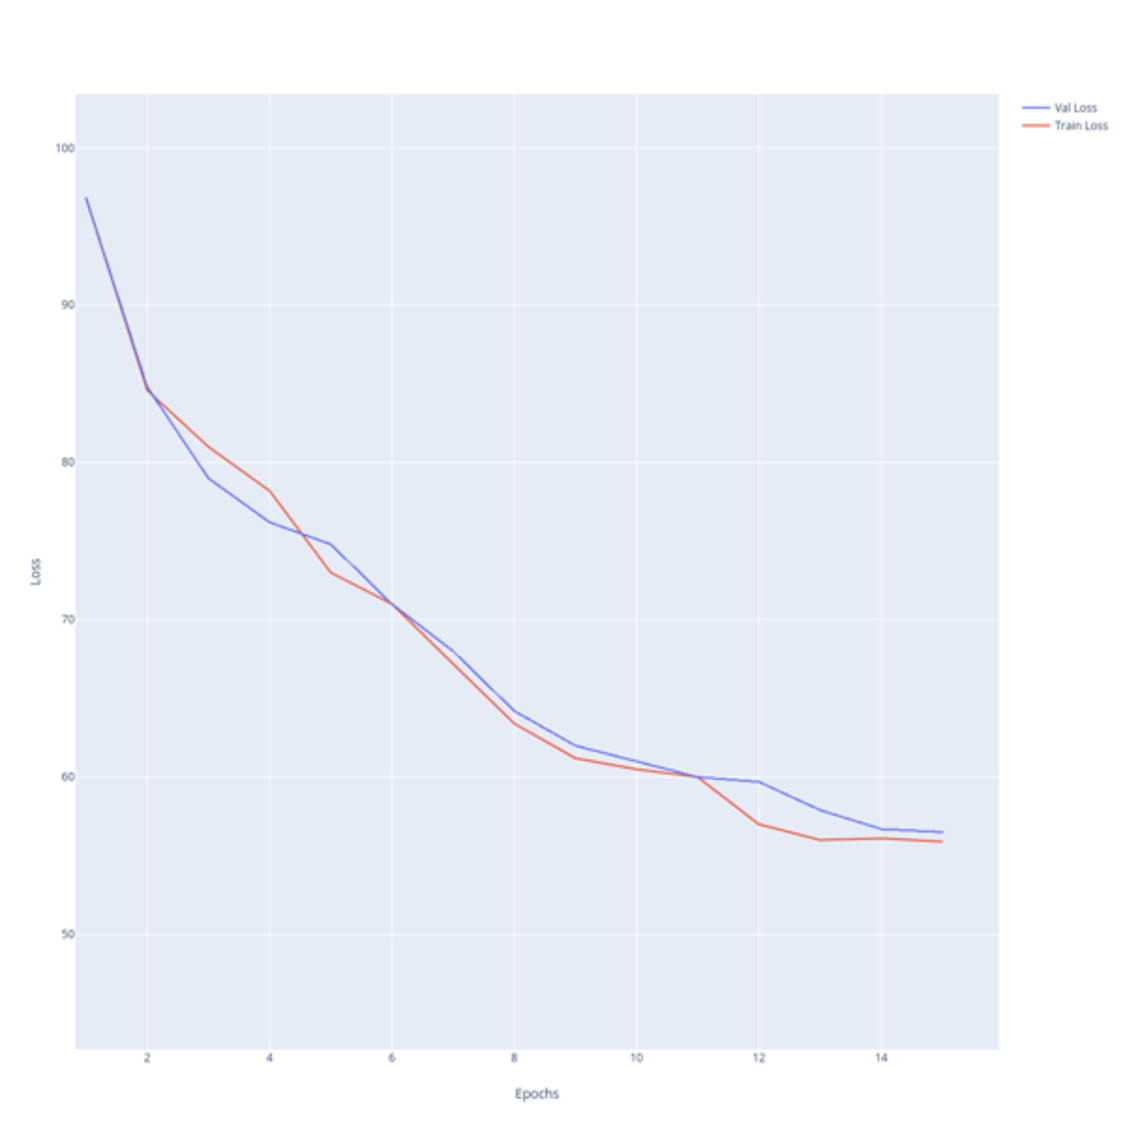
\includegraphics[width=\textwidth]{05-research study/figures/wav2vec2graphloss.pdf}
         \caption{Wav2Vec2 Loss Curves}
         \label{fig:wav2vec2-tl-losscurves}
     \end{subfigure}
     \hfill
     \begin{subfigure}[b]{0.49\textwidth}
         \centering
         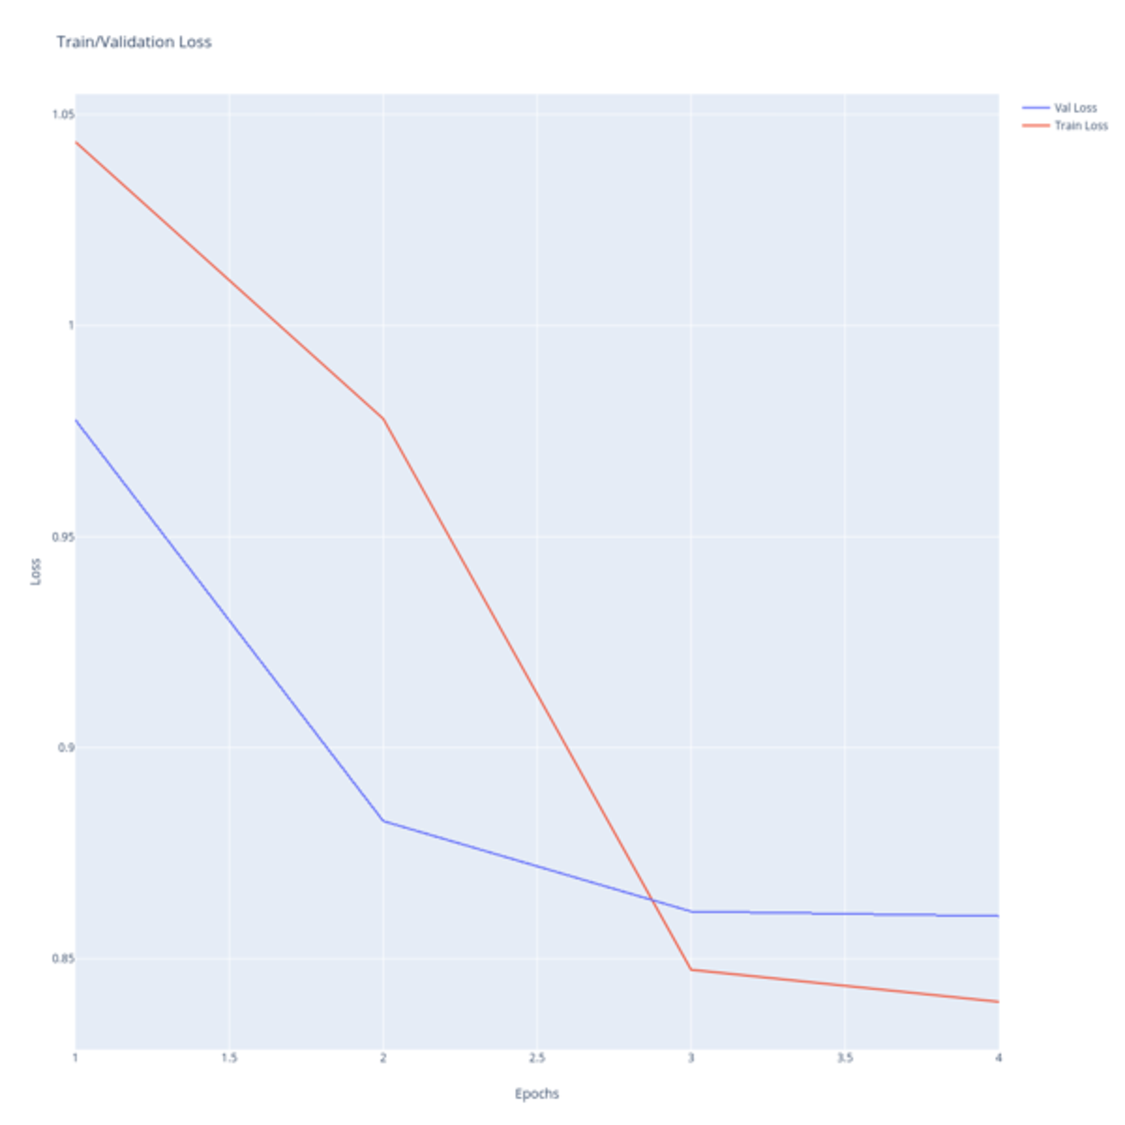
\includegraphics[width=\textwidth]{05-research study/figures/whisperfinetuneloss.pdf}
         \caption{Whisper Loss Curves}
         \label{fig:whisper-tl-losscurves}
     \end{subfigure}
     \hfill
        \caption{Transfer Learning Loss Curves}
        \label{fig:tl-losscurves}
\end{figure}

As seen in figure \ref{fig:tl-losscurves}, the two models are learning effectively from the new domain using fine-tuning approach of transfer learning. The Whisper model's loss curves are quite steep and settle down into a equilibrium before \texttt{EarlyStopping} is activated.

From the above, we have made a lot of improvements on the encoding part of the architectures to be better able to understand the songs domain, we will explore further improvements to be done in the decoding procedure. Our decoding procedure till now has been naive for the Wav2vec2 model as it looks at greedy search only. On the other side, the decoding procedure for Whisper is state of the art, with language identification, beam search and a transformers based decoder architecture all included into the model. Hence, in the next section, we will be implementing improvements that further target the Wav2vec2 architecture mainly.


\subsection{Does beam-search based decoding methods improve the solution?}

In this particular section, we will look at improvements in the decoding architecture. Till now, the Wav2Vec2 architecture has looked at CTC based greedy decoding. As detailed in section \ref{sec:decoders}, there are different types of decoders available that are in the space of Natural Language Processing. Our hypothesis for this section is that we will be able to greatly improve the currrent state of the art by implementing better decoding mechanisms that have knowledge about the lyrics domain. The first improvement that we will see in this particular research question is to see whether Beam Search improves the current best results we have obtained through our research studies.


    \begin{figure}
    \centering
    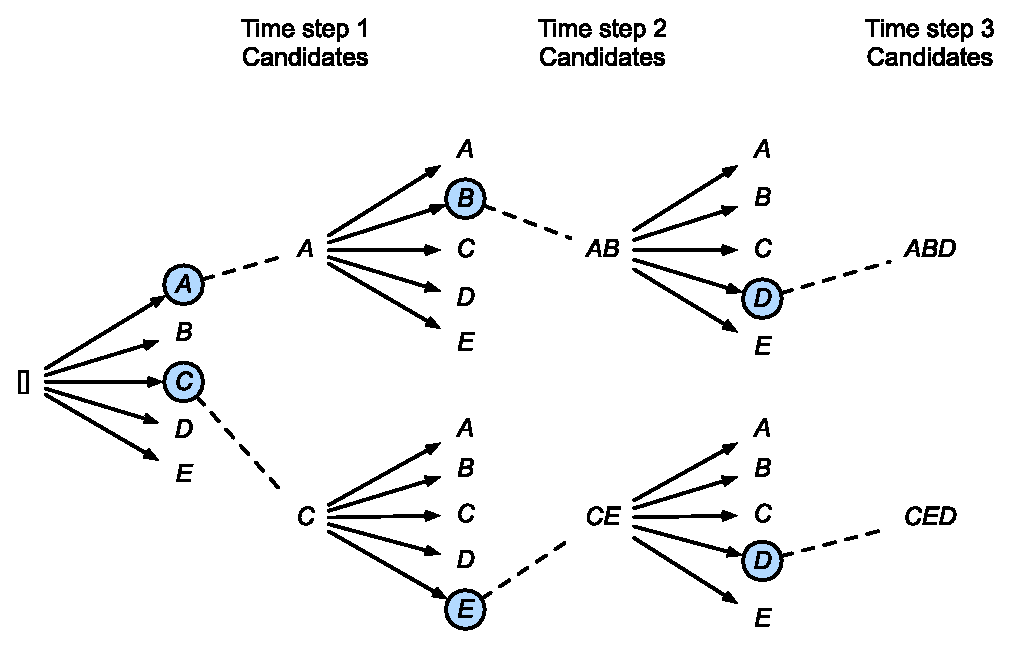
\includegraphics[width=0.7\textwidth]{05-research study/figures/beam-search.pdf}
    \caption{Beam Search \cite{zhang2023dive}}
    \label{fig:beamsearch}
\end{figure}

The Figure \ref{fig:beamsearch} clearly shows the difference between greedy and beam search. The former just takes the highest probable element at each turn and uses Connectionist Temporal Classification(CTC) decoding to create a coherant candidate generation. However, as seen in the figure for beam search, we can choose multiple candidates at each step and then calculate the best overall probability for a sequence of characters to be in the domain of lyrics. Hence, the hypothesis is that the beam search algorithm will significantly improve our current best results as it takes into account multiple candidates. In our study, we took \texttt{beam-size=5} and calculated the WER metric for the validation dataset. The results that were obtained can be seen in table \ref{beamsearch-table}.

In Table \ref{beamsearch-table} onward, we will be referring to \textit{Wav2Vec2 Large Self + SVS + TL} as \textit{Wav2Vec2 Large TL}. Similarly, the model\textit{Whisper Large + SVS + TL} will be referred as \textit{Whisper Large TL}. \\

\renewcommand{\arraystretch}{2}
\setlength{\arrayrulewidth}{0.3mm}
\begin{table}[H]
\small
\begin{center}
\begin{tabular}{ |p{7cm}| p{3cm}| }
\multicolumn{2}{c}{Inference done on \texttt{DALI-validation}} \\
\cline{1-2}
 Models     & WER  \\
\hline  \hline
 \textit{Wav2Vec2 Large TL + Beam Search}   &  0.7346  \\
 \textit{Whisper Large TL}  &  \textbf{0.607}  \\
\hline  \hline
\end{tabular}
\caption{\label{beamsearch-table} Summary of Beam Search Decoder}
\end{center}
\end{table}



From the table, we can see a marginal improvement for the Wav2Vec2 model by implementing Beam Search. When it comes to the Whisper model, beam search is not applied as the model already includes a decoder within it. Hence, there are no improvements that are possible. due to this in the Whisper model. As seen in table \ref{beamsearch-table}, there is only a marginal improvement due to the beam search algorithm. In traditional ASR systems, a lexicon is used along with beam search to give a boost to the words that are there in the target domain. However, with modern approaches, this is rarely done manually and typically is done by leveraging n-gram language models. In the next section, we will create a N-Gram Lyrics Language Model that is trained on the Lyrics domain. Hence, we will use a beam search decoding procedure that gives weightage to both the probabilities from the language model and the acoustic model to come up with the final scores for each candidates at the final step.


\subsection{Does having a lyrics language model improve the solution?}



\begin{figure}
    \centering
    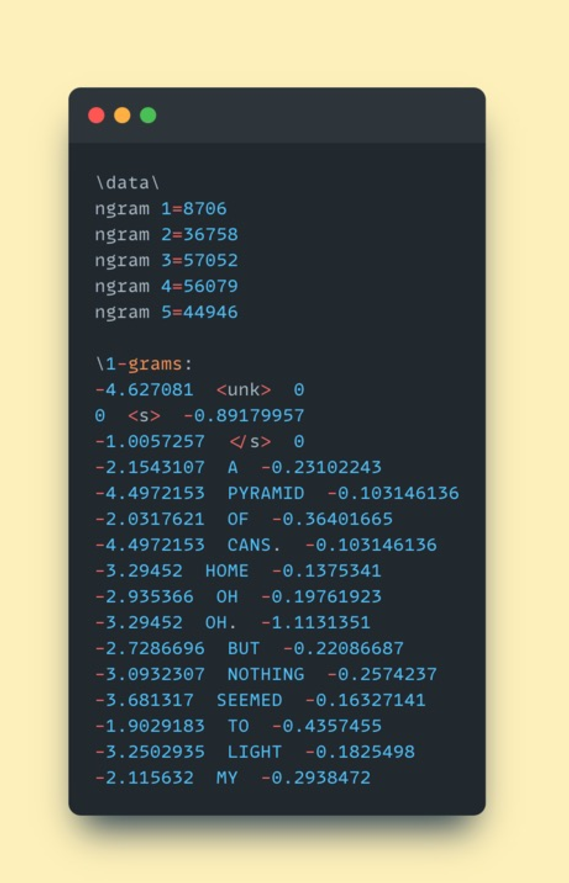
\includegraphics[width=0.4\textwidth]{05-research study/figures/lyricslanguagemodel.pdf}
    \caption{Lyrics 5-gram Language Model}
    \label{fig:lyricslanguagemodel}
\end{figure}


Our goal is to bridge the domain gap between the Speech Transcription to Songs Transcription. In order to do this, we have done music source separation in the input side to bridge the domain gap. By doing so, we have seen that the ASR SoTA models are able to show an improved performance of the songs transcription task. One of the ways end to end ASR system (section \ref{sec:e2easrsystems}) helps to bridge the gap for speech is to have a language model that is aware of the domain while decoding. This helps to perform domain adaptation better. When it comes to the deep learning models, we have seen greedy and beam search based decoder but in both the scenarios, there is no implicit knowledge taken into account about the lyrics domain. Hence, in this section, we will build a statistical language model through the KenLM library \cite{heafield-etal-2013-scalable} that learns up to 5 gram representations of the lyrics within the dataset. When we use the language model within the beam search decoder, we can additionally assign a probability to every sentence on how close it is to the domain (lyrics in our case). We have built a 5 gram model by taking the lyrics in the DALI dataset using the 5-gram model. The Figure \ref{fig:lyricslanguagemodel} shows an excerpt of the language model. For every n-gram, there is an associated probability or score for that particular sequence to be available in that domain. One of the features of KenLM is to use a modified Ksener-Ney smoothing technique on the probability distribution over the n-grams to provide better estimates of probabilities of sentences (any query sentence that did not appear in the training corpus will be assigned zero probability). Additionally, the KenLM model that is produced is memory and time efficient. The method to build it is available in the KenLM GitHub repository.

The output format of the model is \texttt{.arpa} or \texttt{.bin}. We leverage \texttt{pyctcdecode} \cite{KenshoTechnologies} along with the \texttt{lyrics.arpa} 5-gram language model as a decoder. The decoding procedure is built as shown in the below code snippet\cite{KenshoTechnologies}:

\begin{verbatim}
from pyctcdecode import build_ctcdecoder
slt_decoder = build_ctcdecoder(
    labels, #vocabulary
    kenlm_model_path="/lyrics.arpa",  # langauge model path
    alpha=0.4,  # importance of language model
    beta=0.8,  # importance of the acoustic model
)
text = decoder.decode(logits)
\end{verbatim}

The Figure \ref{fig:lyricslanguagemodel} shows an extract from the \texttt{lyrics.arpa} model that has been created by using KenLM. The results shown in the table \ref{ngram-table} are produced with a 5-gram language model as shown in the excerpt and alpha = 0.4 and beta = 0.8.

\renewcommand{\arraystretch}{2}
\setlength{\arrayrulewidth}{0.3mm}
\begin{table}[H]
\small
\begin{center}
\begin{tabular}{ |p{7cm}| p{2cm}| }
\multicolumn{2}{c}{Inference done on \texttt{DALI-validation}} \\
\cline{1-2}
 Models     & WER  \\
\hline  \hline
\textit{Wav2Vec2 Large TL + Beam + LM} &  0.61  \\
\textit{Whisper Large TL} &  0.61  \\
\textit{Whisper Large TL + Post Processing}  & \textbf{0.54}\\
\hline  \hline
\end{tabular}
\caption{\label{ngram-table} 5-gram KenLM Lyrics Model}
\end{center}
\end{table}


From the table \ref{ngram-table}, we can see that the language model boosts the performance of Wav2Vec2 to be on par with the Whisper fine-tuned(Transfer Learning) implementation. Hence, we are able to see a boost in performance by over 17.\% during evaluation. Hence, we can clearly see that the decoder is able to better represent the hidden state outputs from the CTC decoder into the lyrics domain.

In the Whisper model, we see a significant improvement (0.07 WER or 12.96\%) by adding a post-processing layer. The Whisper output has the prediction of \texttt{to} as the first token for some of the predictions. This initial token is followed by correct predictions for the most case. In our study, we simply removed this in the post-processing step. By doing so, we see the 12.96\% improvement in WER metrics.

\subsection{Do Pre-Trained Sequence to Sequence Models/Causal Language Models improve the solution?}

We have seen an improvement of more than 29\% till now from our baseline models through transfer learning and language model implementation. In this particular section, our hypothesis is to take inspiration from this paper \cite{wang2021large} and the Whisper architecture, where encoder-decoder architectures have been successfully implemented to learn Speech to text. The hypothesis is that when applied to Songs to Lyrics transcription problem, we will be able to see a boost in performance because the transformers can learn more complex decoding patterns from the encoder outputs than a n-gram model can learn.

\begin{figure} [H]
    \centering
    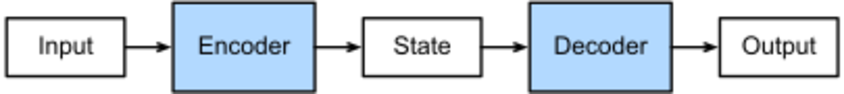
\includegraphics[width=0.7\textwidth]{05-research study/figures/encoder-decoder.pdf}
    \caption{Beam Search \cite{zhang2023dive}}
    \label{fig:encoderdecoder}
\end{figure}



The Sequence to Sequence architecture or Causal Language model can be visualized as an encoder-decoder architecture \ref{fig:encoderdecoder}, where an encoder converts the input signal into a hidden state. On the decoder side, the hidden state is taken and through auto-regressive passing of labels, we aim to get the output that we predict. In our case, the encoder is the pre-trained Wav2Vec2 model or the encoder side of the Whisper model. The decoders we use for the experiment are BertLM  and GPT2 model. The features from the audio signal are extracted based on the methodology of the individual models and sent to the freezed encoder model (no learning happens). The outputs are the logits across the vocabulary space and give the probability of each vocabulary to be the one occurring. In our case, we use the finetuned model as it has adapted to the songs domain the most and is likely to differentiate between the different audio frames or signals. The hidden state is passed to the BertLM or GPT2 along with the labels in an auto-regressive fashion. We enforce teacher forcing methodology \texttt{(teacher-force-ratio = 0.75)} to enable faster convergence. Training is done over 20 epochs and takes 1 GPU around 20 hours to execute. We activate \texttt{EarlyStopping} with a patience value of 3. The results are captured in table \ref{encoderdecoder} . The Wav2Vec2 Encoder and BertLM decoder works the best when using this technique. However, despite the promise in the speech domain, the results are not carrying forward to this particular scenario. Similarly, when we see the GPT2 scenario, the Word Error Rates (WER) do not decrease much and are above 1.

\renewcommand{\arraystretch}{2}
\setlength{\arrayrulewidth}{0.3mm}
\begin{table}[H]
\small
\begin{center}
\begin{tabular}{ |p{7cm}| p{3cm}| }
\multicolumn{2}{c}{Inference done on \texttt{DALI-validation}} \\
\cline{1-2}
 Models     &  WER  \\
\hline  \hline
 \textit{Wav2Vec2 Encoder - BertLM Decoder}            &  \textbf{0.81}  \\
 \textit{Whisper Encoder - BertLM Decoder }           & 0.83 \\
 \textit{Wav2Vec2 Encoder - GPT2 Decoder }        & 1.10 \\
 \textit{Whisper Encoder - GPT2 Decoder}      & 1.10 \\
\hline  \hline
\end{tabular}
\caption{\label{encoderdecoder} Summary of Sequence to Sequence/Causal Models}
\end{center}
\end{table}


\section{Discussion}
\label{sec:discussion-research}

In this chapter, the experiments have been outlined and the evaluation Word Error Rate metrics have been calculated for the experiments that have been conducted. In the next chapter, we will be diving deep into the results obtained and provide analysis on why the results have come out that way. Through the summarization, we will come up with the conclusion for the thesis and future research direction to improve the system even further.
